\chapter{Обзор существующих подходов и теоретическая справка}
\label{cha:ch_1}


\section{Архитектуры нейронных сетей для синтеза речи}
Современные решения для преобразования текста в речь в основном устроены следующим образом: (cм. Рисунок \ref{fig:tts_pipeline})

\begin{enumerate}
    \item В начале текст токенизируется - преобразуется из строкового формата в последовательность лексем - токенов
    \item токенизированный текст преобразуется с помощью нейросети-энкодера во внутреннее признаковое представление
    \item используя текстовые признаки, нейросеть генерирует признаковое представление звука или спектрограмму. Этот модуль может быть многоуровненвым и сложным в зависимости от архитектуры.
    \item признакове представление звука декодируется в звуковой сигнал.
\end{enumerate}

\begin{figure}[t]
  \centering
  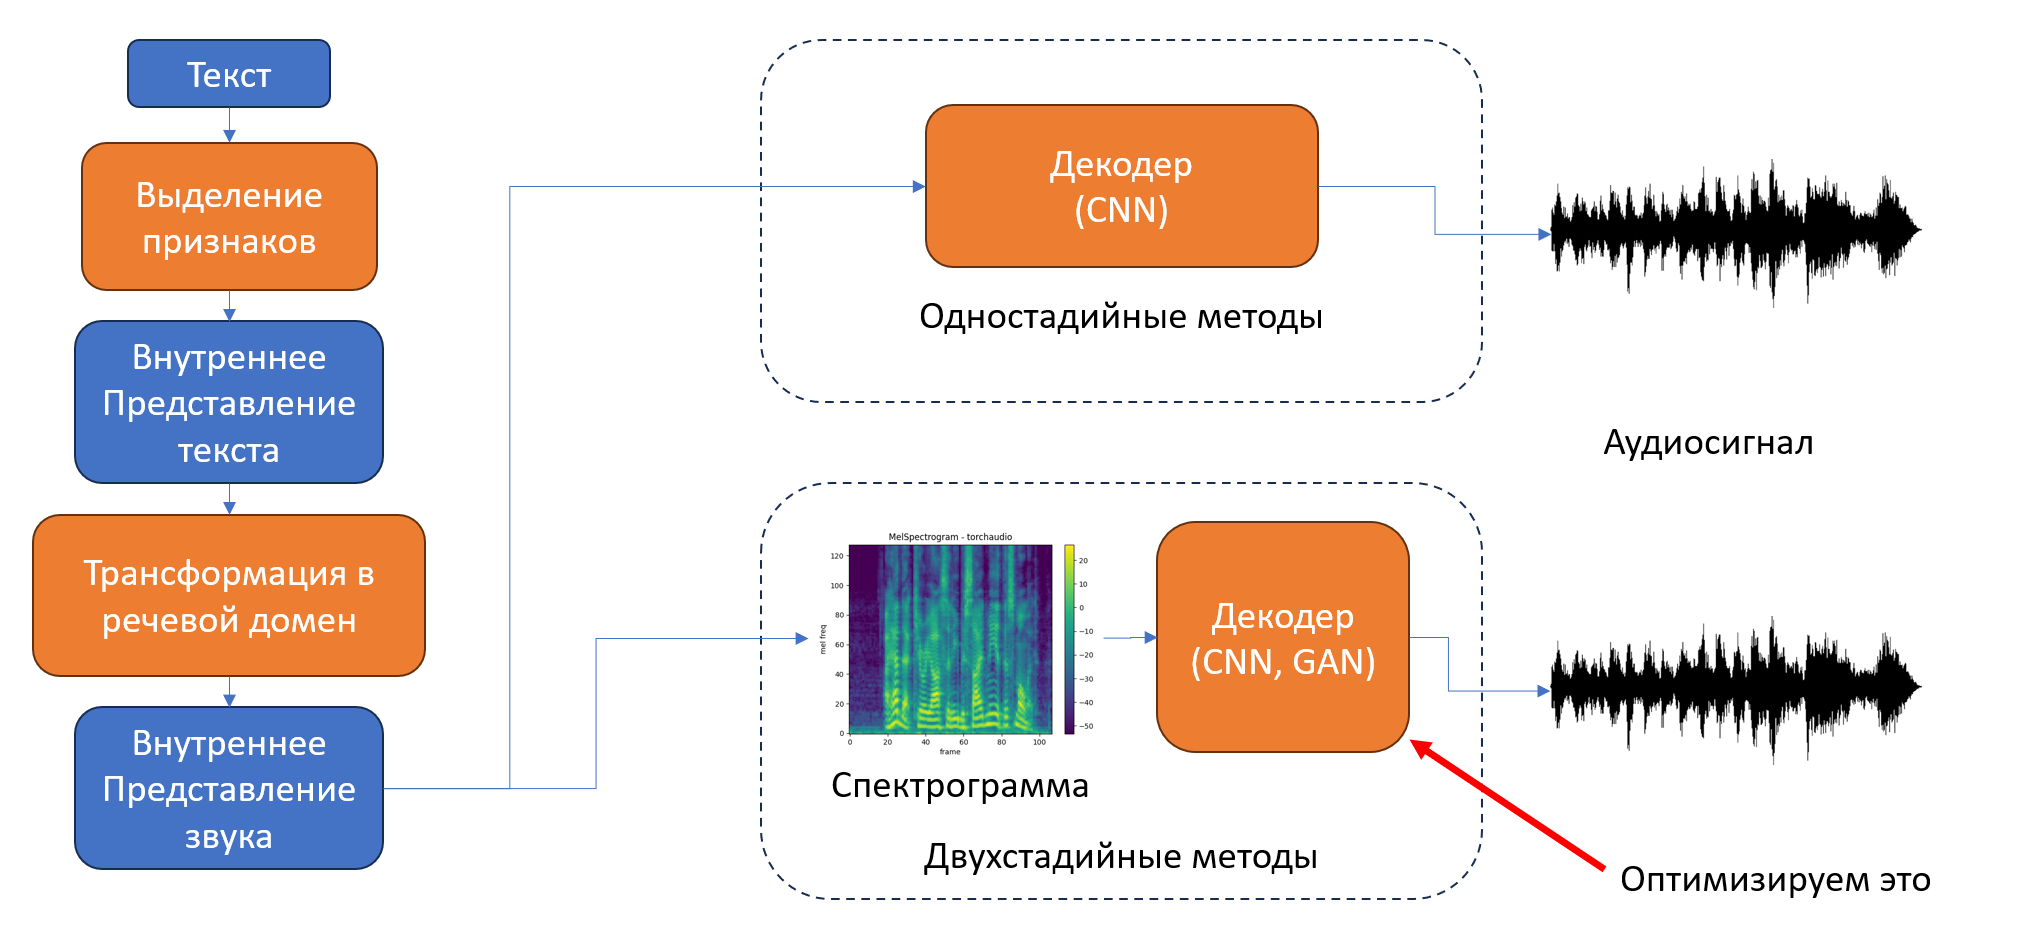
\includegraphics[width=16cm]{figures/tts_pipeline}
  \caption{Преобразование текста в речь}
  \label{fig:tts_pipeline}
\end{figure}

Также помимо задачи преобразования текста в речь, существуют задачи замены голоса, генерации музыки, перевода с сохранением голоса и прочие.
Их пайплайн устроен похожим образом, но какие-то части могут отличаться. 
Отметим, что в любой из перечисленных задач неотъемлемой частью пайплайна является этап декодирования звука из признакового представления в аудиосигнал.

\subsection{Понятие спектрограммы}
Прежде чем продолжить рассмотрение современных подходов для синтеза речи, раскроем понятие спектрограммы.

\textbf{Спектрограмма} - это двумерный массив данных, полученный с помощью оконного преобразования Фурье. 
В результате такого преобразования получается разложение сигнала по частотам в коротко-временном окне, изменяющееся во времени.
По горизонитальной оси отложено время в линейной шкале. По вертикальной оси отложены частоты, в некоторой шкале, не обязательно линейной.
На практике используются линейная, логарифмическая и mel-шкала.
\begin{itemize}
  \item Линейная шкала используется обычно в обратимых алгоритмоах или как разложение для передачи многоканальной информации в одном сигнале.
  \item Логарифмическая шкала используется в музкальных приложениях и редакторах.
  \item Mel-шкала используется для анализа голоса. Она построена на исследованиях чувствительности человеческого слуха к изменению частоты.
\end{itemize}

На рисунке \ref{fig:log_spec} изображен пример спектрограммы в логарифмической шкале, а на рисунке \ref{fig:mel_spec} - в mel-шкале.
\begin{figure}[t]
  \centering
  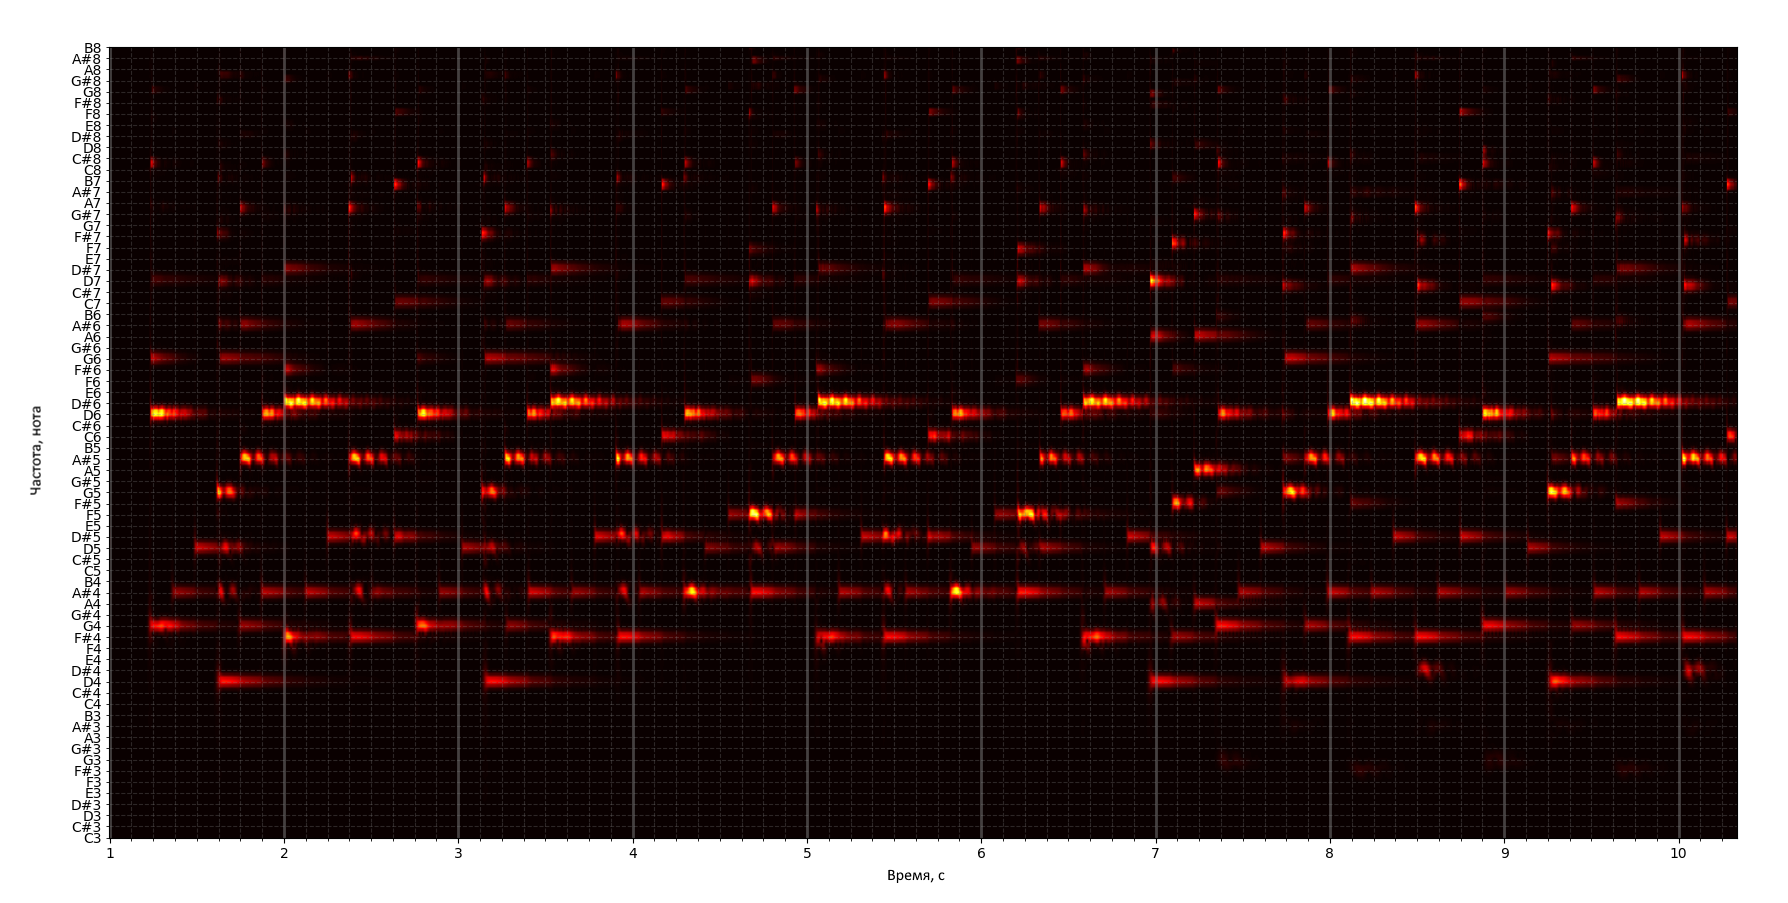
\includegraphics[width=16cm]{figures/log_spec}
  \caption{Спектрограмма записи игры на металлофоне в логарифмической шкале частот с указанием нот}
  \label{fig:log_spec}
\end{figure}

\begin{figure}[t]
  \centering
  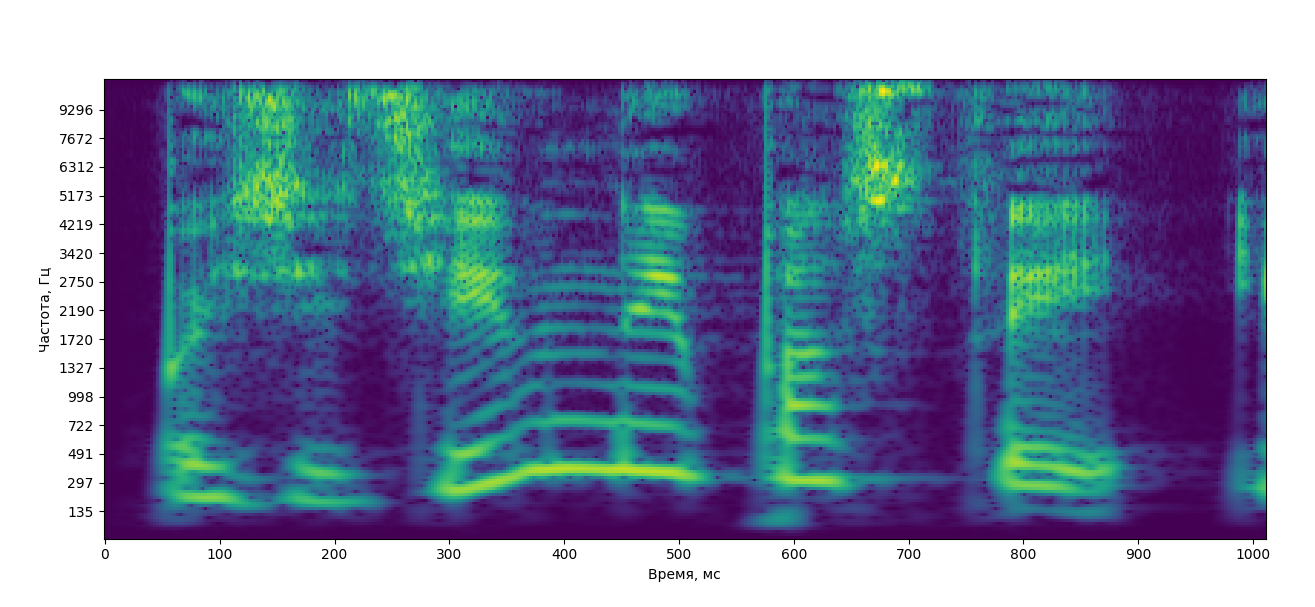
\includegraphics[width=16cm]{figures/mel_spec}
  \caption{Спектрограмма записи голоса в mel-шкале}
  \label{fig:mel_spec}
\end{figure}

\subsection{Классификация подходов}
Рассмотрим основные подходы, использующиеся в современных решениях синтеза речи и их условную классификацию.

По принципу использования спектрограммы методы делятся на двухстадийные и одностадийные (end-to-end):
\begin{itemize}
    \item Двухстадийные методы подразумевают генерацию спектрограммы с последующим преобразование спектрограммы в звуковой сигнал.
    \item одностадийные методы.
\end{itemize}

\subsubsection{Двухстадийные методы - генерация спектрограммы}
Tacotron 2: Классическая модель, использующая последовательное преобразование текста в мел-спектрограмму с последующим применением вокодера
FastSpeech 2: Улучшенная версия FastSpeech, обеспечивающая высококачественный синтез речи с контролем над длительностью, высотой тона и энергией
\subsubsection{Одностадийные методы - Wav2Vec}
\subsubsection{Трансформерные генераторы}
\subsubsection{Диффузионные генераторы}
\subsubsection{Мультимодальные LLM-генераторы}
\subsubsection{Полносверточные сети}




 - какие есть
   - диффузия
   - трансформер
   - unet для замены голоса
   - wav2vec
   - одностадийные, двухстадийные
 - понятие спектрограммы
 - примеры, ссылки
 - проблемы для каждой
 - сравнение, преимущества и недостатки, сферы применения

\section{Cуществующие вокодеры}
 - Существующие Вокодеры
  - GriffinLim (algo) \cite{1164317}
  - WaveGlow (gan)
  - EnCodec
 - Приемущества и недостатки существующих вокодеров 
 - примеры генерации от вокодеров, проблемы с ними
 - Алгоритм Гриффина-Лима
  - верхнеуровневое описание
 - нейросеть привязана к домену, на котором училась, алгоритм не привязан, но могут быть артефакты
 - быстродействие алгоритма и нейросети

\section{Представление и анализ аудиосигналов}
 - оконное преобразование Фурье
 - принцип неопределенности в пространстве частота-время
 - окна
 - децибел шкала амплитуд
   - почему такая
   - формула
   - порог слышимости
 - мел шкала
   - почему такая
   - формула
 - выбор оптимальной шкалы частот
  - линейная шкала
  - логарифмическая шкала
  - мел шкала
  - комбинированная шкала
 - избыточность информации в спектрограмме
 - наложение по времени
 - наложение по частоте
 - оптимальный размер окна для конкретной шкалы частот
 - сравнение с вейвлетами
 - восстановление сигнала с наложением (суммирование, сумма дает 0 там где надо, но хвосты могут расползаться)
 - оптимальная форма окна для устойчивости к искажениям
   - минимизация связанности далеких данных
 - Алгоритм Гриффина-Лима
    - как работает

 \section{Устойчивость к трансформациям и артефактам}
 - трансформации спектрограммы, устойчивость вокодера к трансформациям
   - растяжение\сжатие по времени
   - перемещение по шкале частот
   - вырезание\вставка куска
   - суммирование сигналов
 - от чего появляются трансформации и зачем нужны
 - артефакты от нейросетей
   - примеры полосок от сверток
   - BatchNorm паразитный bias
   - потеря шума
   - потеря outliers
 - устойчивость вокодеров к артефактам
 - инвариантность к сдвигу по времени, когда есть, зачем нужна

\section{Открытые проблемы}
 - борьба за качество генерации
 - как восстанавливать сигнал с нелинейной шкалой частот, когда нет ортогонального базиса
 - нет алгоритма, который был бы достаточно устойчив к артефактам от нейросетей
 - нейросетевые вокодеры:
   - требуют вычислительных ресурсов
   - нужно обучать на больших объемах данных
   - часто завязаны на домен, для другого домена могут хуже работать
 - избыточность представлений, тащим лишнюю информацию
 - нужна устойчивость обучения, глубокие сети сложнее учить

\section{Выводы по главе}

